\chapter{\hisparc Experiment}
\label{ch:hisparc-experiment}

Detecting cosmic-ray extensive air showers with affordable detectors
using plastic scintillators and photomultiplier tubes, the design is
explained in \secref{sec:detector_design}.

Large network area, sparse array. Detector station locations are often
limited to high-school roofs or universities and other institutions.
Some stations, however, are located at the homes of participants, e.g.
a garage roof [photo nijmegen/ucu?].


\section{Network status}

Currently there are 120 active \hisparc stations in the world. Stations
are located at high schools and research institutes in the Netherlands,
United Kingdom and Denmark.

[plot for number of active stations from 2004-ish untill now]


\begin{figure}
    \centering
    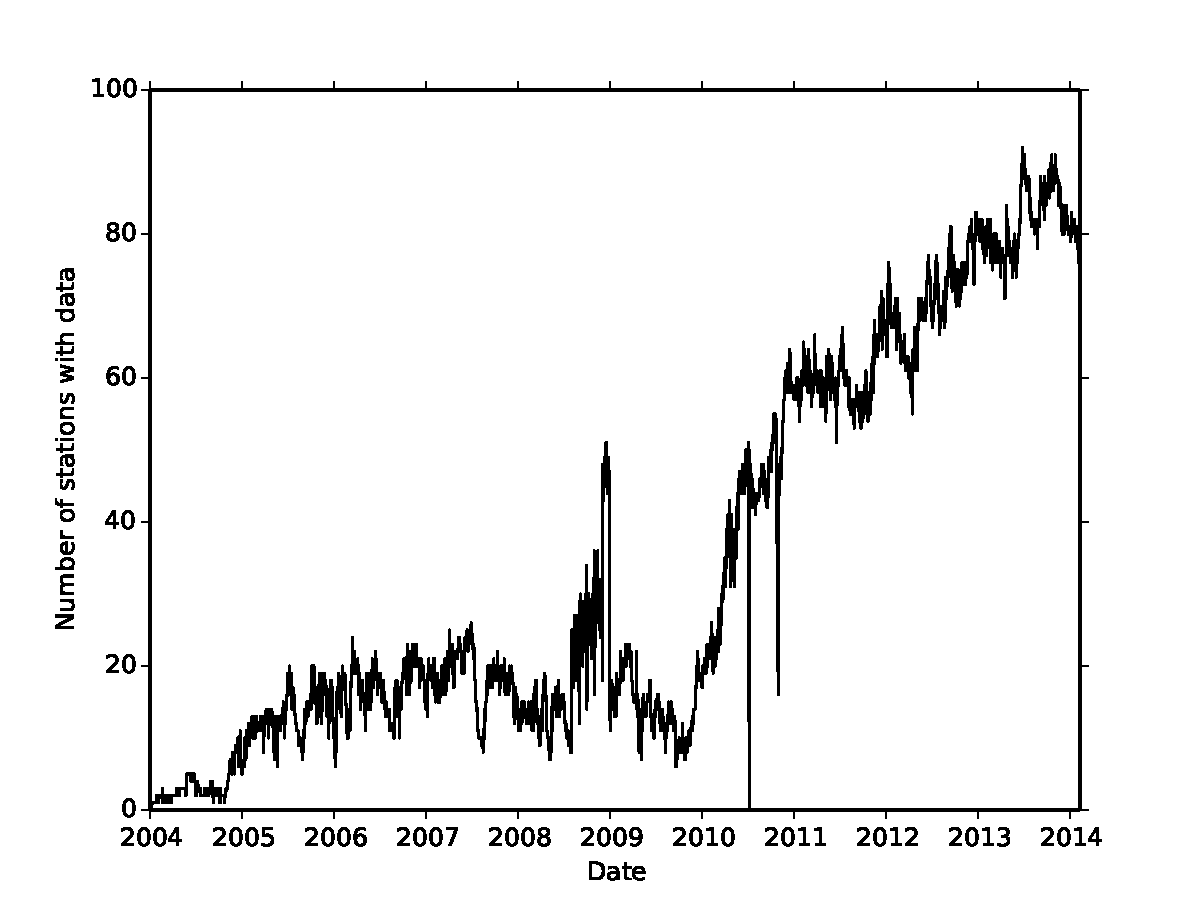
\includegraphics[width=0.7\linewidth]{plots/network/number_of_stations_with_data_per_day}
    \caption{\captitle{Active stations over time.} The number of active
             stations per day from January 1st 2004 until now.}
    \label{fig:number_of_stations_with_data_per_day}
\end{figure}


\subsection{International}

In Germany one of our stations (70001) was placed inside the \kascade
experiment in Karlsruhe on July 1, 2008. This was done to calibrate and
test the direction reconstruction accuracy of a single \hisparc station.
Although the \kascade-GRANDE experiment officially shut down on March
30, 2009, it was kept active until November, 26th 2011 as a test
facility for some test setups, including our detector. The \kascade
experiment triggered the \hisparc station when it detected a shower. It
was triggered more than \num{9e7} (in publicdb, more on external hdd?
and in `/databases/kascade`?) times in this period. The detectors have
been repurposed and are now part of station 508 on the Science Park.

Since 2007 there has been a \hisparc station in
Denmark. There are currently 3 operational stations at the Aarhus
University. These stations are managed by Uffe Amelung Fredens.
Fredens is writing student materials for Danish high school students.

In Bristol, England a new cluster started to form around Bristol in
March 2012. This was initiated by Dr. Jaap Velthuis who is the cluster
coordinator for Bristol. Since then schools in Bristol, Bath, Swindon
and Chippenham have joined the network. More on the way..

[Finland/Spain.. perhaps?]


\section{Detector design}
\label{sec:detector_design}

\subsection{Scintillator}

\SI{100 x 50 x 2}{\centi\meter} cuboid of plastic scintillator, with the
base polyvinyltoluene and the fluor anthracene.


\subsection{Photo multiplier}

Performance
Nikhef designed high-voltage voltage-divier circuit.
Cockcroft-Walton voltage multiplier circuit.
High linearity?


\subsection{HiSPARC III}

Readout electronics. Two channels, each with two ADCs which readout a
signal up to \SI{-2}{\volt}. And return a 12-bit value (4096 ADCcounts
range). Each ADC is sampled at 200 Mhz, using two ADCs per channel gives
400 Mhz (2.5 ns) per channel. Nikhef designed. Some (derivatives) used
in other experiments.

Latest version \hisparc III. New software needed, easier firmware updates.
